
\section{Why Residual Error Misleads}
\label{sec:mechanism}

\paragraph{Injection structure changes the error recursion.}
Let $\delta_b$ be the deviation of the cached branch from the exact trajectory at
block $b$. Under plain caching the reused residual $R_{a,b}$ is a \emph{constant}
with respect to the current state, so
\begin{equation}
\delta_{b+1} = \delta_b + \big(R_{a,b} - R_b(h^\star_b)\big),
\label{eq:additive}
\end{equation}
and deviations \emph{add} along depth. A corrector that works restores state
dependence, $\mathrm{out}_b \approx h_b + R_b(h_b)$, which linearises to
\begin{equation}
\delta_{b+1} \approx (I + J_b)\,\delta_b + \varepsilon_b,
\qquad J_b = \partial R_b / \partial h,
\label{eq:multiplicative}
\end{equation}
so deviations \emph{multiply}. The more faithfully $C$ imitates the true block, the
larger the feedback gain it reintroduces. Consequently the number of injection sites
per step, not the accuracy at each site, dominates stability.

This yields a falsifiable prediction: coarsening the injection granularity should
\emph{degrade} residual accuracy while \emph{improving} deployed quality.
Table~\ref{tab:granularity} is consistent with it. Splitting the $B{=}28$ stack into
$K$ cached segments leaves the correction-free baseline unchanged
(Sec.~\ref{sec:setup}), so all rows share one reference. We must flag that the rows
are \emph{not} matched correctors: each $K$ has its own trained model, differing in
width/depth/rank, parameter count ($11.9$--$21.3$M) and step budget, and $K{=}28$ pays
$28$ corrector calls per reuse step rather than one. The ladder is therefore
suggestive, not controlled; we use it only for the qualitative direction. The
controlled evidence for the aggregation argument is Sec.~\ref{sec:inversion}, where
everything but the loss is fixed.
Residual accuracy is best at $K{=}28$ by a factor of six; at full injection strength
deployed quality is ordered strictly the other way, and the least accurate corrector,
$K{=}1$, is the only granularity that yields a real gain. Damping can rescue the
finest granularity to approximately neutral --- at $\sigma{=}0.2$, $K{=}28$ reaches
$+0.0087$ --- which is consistent with the mechanism: shrinking the injected
correction shrinks the feedback gain it reintroduces, at the cost of most of the
correction.

\begin{table}[t]
\centering\small
\begin{tabular}{rrrrr}
\toprule
 & & & \multicolumn{2}{c}{SSIM vs.\ plain caching} \\
\cmidrule(l){4-5}
$K$ & blk/seg & val $\relmse$ & at $\sigma{=}1$ & best $\sigma$ \\
\midrule
28 & 1  & \best{0.0537} & $-0.3115$ & $+0.0087$ \\
4  & 7  & 0.2021        & $-0.2509$ & $-0.0304$ \\
2  & 14 & 0.2724        & $-0.2352$ & $-0.0036$ \\
1  & 28 & 0.3166        & \best{$+0.0516$} & \best{$+0.0713$} \\
\bottomrule
\end{tabular}
\caption{Injection granularity moves the two metrics in opposite directions. At
matched injection strength ($\sigma{=}1$, no selection) quality is monotone in the
number of injection sites. The best-$\sigma$ column is \emph{selected on the same
$n{=}8$ design split it reports} and is therefore optimistic --- we include it only to
show that damping rescues fine granularity to roughly neutral rather than to a gain;
with per-prompt SD $\approx0.12$ its standard error is $\approx0.04$, so individual
entries there are not separately meaningful. Plain caching scores $0.3868$.
Note also that $\relmse$ is \emph{not} comparable across rows: the target is a
per-block $\dR$ at $K{=}28$ and a whole-stack $\dR$ at $K{=}1$. This table therefore
supports the granularity mechanism (Eq.~\ref{eq:multiplicative}), not the
aggregation argument, for which see Sec.~\ref{sec:inversion}.}
\label{tab:granularity}
\end{table}

\begin{figure*}[t]
\centering
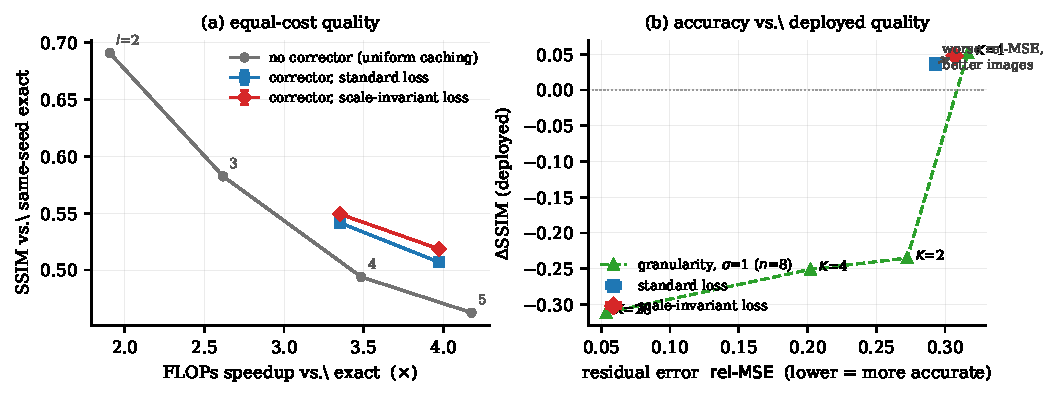
\includegraphics[width=\textwidth]{figs/front.pdf}
\caption{\textbf{(a)} Learned correction lifts the equal-cost front; the
scale-invariant objective lifts it further at both operating points, with identical
architecture, parameter count and wall clock. Points are $n{=}192$ held-out images;
per-image paired statistics and clustered intervals are in Table~\ref{tab:main}. Error bars are the spread
over three training seeds. \textbf{(b)} The two metrics are anti-correlated along
both axes we can vary: injection granularity (green, residual accuracy improves
$6\times$ from $K{=}1$ to $K{=}28$ while quality collapses) and the training
objective at fixed granularity (blue $\rightarrow$ red, residual error gets worse and
images get better). No point in this figure is consistent with using residual error
to select a corrector.}
\label{fig:front}
\end{figure*}

\paragraph{Is it really feedback, or just a mis-scaled corrector?} Eq.~\ref{eq:multiplicative}
invites an objection: a \emph{perfectly} faithful corrector reproduces the exact
stack's own dynamics, and the exact model does not diverge, so ``more faithful implies
less stable'' cannot follow from the recursion alone. A simpler explanation is
available in our data --- the per-block corrector over-predicts at $\tau{=}1$, with
$\lVert\hat{\dR}\rVert/\lVert\dR\rVert$ of $1.50, 1.11, 1.10, 1.15$ across the four
anchor cycles (mean $1.22$; at $\tau\ge2$ it slightly \emph{under}-predicts) --- and
even a $1.2\times$ gain error compounded over $28$ blocks would destroy the image by
itself. That would
make the granularity collapse a \emph{calibration} defect, trivially fixable by
rescaling, rather than evidence about metric aggregation.

We tested it directly by sweeping the scalar gain on the $K{=}28$ corrector
(Table~\ref{tab:calib}). The calibration hypothesis predicts a rescue near
$\sigma = 1/1.5 \approx 0.67$. Instead $\sigma{=}0.667$ produces SSIM $0.302$ against
plain caching's $0.597$, and the best value any scalar gain achieves is $\sigma{=}0.1$,
which merely turns the corrector off ($+0.0005$). No scalar calibration recovers
anything, while $K{=}1$ on the same split gains $+0.0500$. Degradation is smooth and
monotone in $\sigma$, with collapse well before full injection --- the signature of a
gain that amplifies with the size of what is injected, not of a constant mis-scaling.
We take this as support for the recursion argument, while noting we still do not
measure $J_b$ or its spectral radius directly.

\begin{table}[t]
\centering\small
\begin{tabular}{rrrr}
\toprule
$K{=}28$ at $\sigma$ & SSIM & vs.\ plain & vs.\ $K{=}1$ \\
\midrule
0.1   & 0.5973 & $+0.0005$ & $-0.0495$ \\
0.3   & 0.5797 & $-0.0171$ & $-0.0672$ \\
0.5   & 0.4991 & $-0.0976$ & $-0.1477$ \\
$0.667^{\ast}$ & 0.3019 & $-0.2949$ & $-0.3449$ \\
1.0   & 0.0438 & $-0.5530$ & $-0.6030$ \\
\bottomrule
\end{tabular}
\caption{No scalar gain calibration rescues per-block injection. $^{\ast}$is the value
predicted by the measured $1.5\times$ over-prediction; it is catastrophic. Plain
caching scores $0.5968$ and the $K{=}1$ corrector $0.6468$ on this split
(val, $n{=}24$).}
\label{tab:calib}
\end{table}

\paragraph{Energy weighting.} The recursion above explains granularity but not why
$\relmse$ misranks two correctors at \emph{fixed} granularity. That comes from how
Eq.~\ref{eq:relmse} aggregates. It sums squared error and target energy over sites
separately, so a site contributes in proportion to $\lVert\dR\rVert^2$. Target
magnitude grows steeply with the distance $\tau$ from the anchor: on our primary
backbone the per-site target RMS is $1.00, 1.64, 2.35, 3.30$ for
$\tau = 1,2,3,4$, so $\tau{=}4$ sites carry $\approx\!11\times$ the squared energy of
$\tau{=}1$ sites and dominate both the metric and --- if one trains on the same
aggregation --- the gradient.

Deployment does not share that weighting. Every injection site feeds the \emph{same}
propagation chain, and Eq.~\ref{eq:multiplicative} does not care whether the site's
target was large or small; only the \emph{relative} fidelity of the injected
correction matters. Worse, errors at small $\tau$ propagate through the remaining
steps of the anchor cycle, so the sites $\relmse$ discounts most are the ones whose
errors compound longest. This predicts that (i) an objective which weights sites
equally should deploy better while scoring worse on $\relmse$, and (ii) a
\emph{per-site} relative statistic should track deployment where $\relmse$ does not.
Sections~\ref{sec:loss} and \ref{sec:proxy} test both.

\section{Experiments}

\subsection{A scale-invariant objective}
\label{sec:loss}

The standard objective divides the target by a single global scale $\hat{s}$ and
applies a plain MSE, $\mathcal{L}_{\text{std}} = \lVert \hat{\dR}/\hat{s} - \dR/\hat{s} \rVert^2$,
which inherits exactly the energy weighting of Eq.~\ref{eq:relmse}. We compare it
against a per-site normalisation,
\begin{equation}
\mathcal{L}_{\text{inv}} = \Big\lVert \big(\hat{\dR} - \dR\big) \big/ \max(\lVert \dR \rVert_{\text{rms}}, \epsilon) \Big\rVert^2 ,
\label{eq:invloss}
\end{equation}
which optimises relative error per site. Everything else is held fixed: same data,
same architecture, same parameter count, same injection structure, same FLOPs.

Table~\ref{tab:main} reports the outcome on $192$ held-out images. Two things should
be read from it in order of confidence.

First, \textbf{correction works, robustly}. Every corrected variant beats plain caching
at the same anchor schedule with paired $t$ between $9.9$ and $19.3$, improving
$149$--$182$ of $192$ images, and it does so on all three metrics we measure plus CLIP
similarity (Sec.~\ref{sec:clip}). At $3.97\times$ FLOPs reduction the best corrector
gains $+0.0507$ SSIM over the equal-cost correction-free front. This is not the
paper's point but it is its firmest measurement.

Second, \textbf{the loss matters, but by little}. In the design we trust --- arms
step-matched at $16$k with no checkpoint selection, three seeds each, damping chosen on
validation --- the scale-invariant objective gains $+0.0077$ SSIM and $-0.0091$ LPIPS,
both significant under subject clustering ($t(5){=}2.74$, $-3.18$). Meanwhile
$\relmse$ prefers the standard loss in all three seeds with non-overlapping ranges
($0.330$--$0.333$ against $0.334$--$0.336$). That is the inversion in its cleanest
form: the residual metric separates the arms crisply and points the wrong way, while
the image metrics separate them weakly and point the right way. Across every condition and metric the sign is the same, and a
corrector trained on \emph{half} the data with the better loss ($+0.0431$) still beats
one trained on twice the data with the standard loss ($+0.0363$). What we cannot do is
put a tight number on it: with six held-out subjects, effects of this size sit near our
measurement resolution, and our successive estimates fell from $+0.0217$ to $+0.0077$
as we removed uncontrolled degrees of freedom (Sec.~\ref{sec:limits}).

This is why the paper's claim is the \emph{ordering}, not the magnitude. The ordering
is what contradicts $\relmse$, and the ordering is stable across samples, metrics,
seeds and data conditions; the magnitude is not.

\begin{table}[t]
\centering\small
\begin{tabular}{llrrr}
\toprule
design & metric & effect & paired $t$ & cluster $t(5)$ \\
\midrule
\multicolumn{5}{l}{\emph{step-matched, 3 seeds/arm, no checkpoint selection:}}\\
clean & SSIM  & \best{$+0.0077$} & $3.69$ & \best{$2.74$} \\
clean & LPIPS & \best{$-0.0091$} & $-3.53$ & \best{$-3.18$} \\
\midrule
\multicolumn{5}{l}{\emph{other designs, each confounded as noted:}}\\
union $2\times$ & SSIM  & $+0.0115$ & $3.16$ & $0.96$ \\
union $2\times$ & LPIPS & $-0.0299$ & $-6.78$ & $-3.12$ \\
base, selected$^\dagger$ & SSIM & $+0.0266$ & $9.75$ & $3.85$ \\
base, selected$^\dagger$ & LPIPS & $-0.0039$ & $-1.14$ & $-1.34$ \\
\bottomrule
\end{tabular}
\caption{The loss contrast (scale-invariant $-$ standard) at matched data,
architecture, parameter count and cost. All rows: $192$ held-out images ($24$ prompts,
$6$ unbalanced subject clusters of $8$--$40$ images, $8$ image seeds); clustered
intervals are percentile bootstraps ($20{,}000$ resamples) and the cluster $t$ is the
more conservative statistic on cluster means. \textbf{The first block is the design we
rely on}: both arms trained to the same step with no validation-based checkpoint
selection, three seeds each, one damping per arm chosen on validation and averaged over
seeds. Both metrics are significant there, with CIs $[+0.002,+0.015]$ and
$[-0.015,-0.003]$. $^\dagger$This row's arms were checkpoint-selected by validation
$\relmse$ and landed on different steps ($6$k vs.\ $12$k of $16$k) --- selecting by the
metric this paper indicts --- so its larger effect should not be trusted; we show it
because an earlier draft of this work headlined it. Per-arm seed ranges overlap in the
clean design ($+0.034$--$+0.045$ std, $+0.041$--$+0.054$ inv), so unlike an earlier
draft we make no ``non-overlapping ranges'' claim. Correction itself remains far larger
than the choice of loss: $+0.034$ to $+0.054$ SSIM over plain caching at the same
anchor schedule.}
\label{tab:main}
\end{table}

\subsection{Does the effect scale with the imbalance?}
\label{sec:scaling}

The mechanism makes a quantitative, pre-measurable prediction: the fix corrects an
imbalance in per-site contribution, so its benefit should grow with how imbalanced the
sites are --- a quantity computable from the collected data before any corrector is
trained. Table~\ref{tab:scaling} tests it across the three conditions we have. The
cleanest of the three is internal: anchor interval $4$ versus $5$ on the \emph{same}
backbone, same data and same architecture, differing only in that $i{=}4$ spans
$\tau \in \{1,2,3\}$ and therefore has a $2\times$ smaller energy spread. Its loss
effect is correspondingly smaller, and the ratio of effects ($1.49$ at $n{=}192$)
tracks the ratio of imbalances ($1.40$) closely --- though with both effects now near
the resolution of our data, we present the ordering rather than the ratio as the
claim.

\begin{table}[t]
\centering\small
\begin{tabular}{llrrr}
\toprule
backbone & $i$ & $\lVert\dR\rVert$ ratio & energy & loss effect \\
\midrule
primary & 5 & $3.30$ & $10.9\times$ & $+0.0115$$^\ddagger$ \\
primary & 4 & $2.35$ & $5.5\times$  & $+0.0077$ \\
FLUX    & 5 & $1.92$ & $3.7\times$  & $\approx 0$ (n.s.) \\
\bottomrule
\end{tabular}
\caption{The benefit of per-site normalisation tracks the per-site target-energy
imbalance it corrects. Columns 3--4 are properties of the \emph{data}, measurable
before training. Rows 1--2 differ only in anchor interval on one backbone and are
thus a controlled test; row 3 additionally changes backbone and tokens-per-site, so it
corroborates rather than isolates. $^\ddagger$For comparability across rows these are all union-data
effects, so row 1 is the $+0.0115$ union figure rather than the $+0.0077$ figure from
the step-matched design. Three points cannot establish a scaling law, but they are ordered as the mechanism
requires, and the relation is falsifiable on any
new backbone at the cost of one feature-collection pass.}
\label{tab:scaling}
\end{table}

We emphasise what this does and does not establish. It was constructed after seeing
the FLUX negative result, so it is an account rather than a confirmed prediction, and
row 3 is confounded. But rows 1--2 are a clean within-backbone test that we did not
have to run --- the numbers were already in the $2\times2$ --- and they come out in the
predicted direction with roughly the predicted magnitude. The practical implication is
concrete: measure the spread of $\lVert\dR\rVert$ across $\tau$ first, and expect the
scale-invariant objective to be worth roughly nothing when that spread is flat.

\subsection{The inversion}
\label{sec:inversion}

Table~\ref{tab:inversion} places the two metrics side by side for the replicated
contrast. Every one of the three scale-invariant runs scores worse on $\relmse$ and better on
images than every one of the three standard-loss runs. $\relmse$ is not a noisy proxy
here; it is a precise instrument pointing the wrong way.

We deliberately do not call this ``$9$ independent pairs''. The $3\times3$ outcomes
follow deterministically from one rank separation between two arms of three runs; the
correct statement is a single rank separation (exact permutation floor $p{=}0.05$ for
$3$-vs-$3$) reinforced by the per-image paired test ($t{=}4.5$, subject-clustered CI
excluding zero) and by agreement across metrics: on the loss axis SSIM, LPIPS
\emph{and} PSNR all prefer the scale-invariant corrector. That last check rules out
the obvious alternative --- that per-site normalisation merely smooths output in a way
SSIM rewards. On the \emph{data} axis the three metrics disagree (SSIM prefers the
union set, LPIPS and PSNR the base set), a further reason we treat the data effect as
unresolved.

\begin{table}[t]
\centering\small
\begin{tabular}{lccc}
\toprule
loss & $\relmse\downarrow$ & per-site med.$\downarrow$ & $\Delta$SSIM$\uparrow$ \\
\midrule
std & \best{0.2924 / 0.2929 / 0.2929} & 0.573--0.574 & $+0.0305$ \\
inv & 0.3064 / 0.3069 / 0.3073 & \best{0.564--0.566} & \best{$+0.0522$} \\
\midrule
\multicolumn{4}{l}{\emph{agreement with image ranking:} $\relmse$ 0/9, per-site 9/9}\\
\bottomrule
\end{tabular}
\caption{Residual error prefers the standard loss on all three seeds; images prefer
the scale-invariant loss on all three. Image column is $\Delta$SSIM vs.\ the
equal-cost front, $n{=}48$ (the $48$-image sample; see Table~\ref{tab:main} for the
$n{=}192$ figures we now prefer). The per-site median relative error agrees with
images.}
\label{tab:inversion}
\end{table}

\subsection{A proxy that does track deployment}
\label{sec:proxy}

Replacing the energy-weighted aggregation of Eq.~\ref{eq:relmse} with a per-site
statistic --- the median over sites of $\lVert \dR - \hat{\dR}\rVert / \lVert \dR \rVert$
--- yields a metric that needs no image generation and ranks correctly. Across ten
checkpoints with deployment numbers it agrees with the image ranking on every
same-training-set pair whose deployed difference exceeds the seed noise. This is
weaker evidence than the count suggests and we say so: most such pairs \emph{are} the
loss contrast that motivated the statistic, leaving few independent same-data
comparisons, and the noise filter conditions on the outcome variable by removing
near-ties. Treat it as a hypothesis with supporting evidence, not a validated
criterion.

It is not a universal replacement. Across \emph{different} training sets it fails on
$6$ of $26$ pairs, and the failures are systematic: every one under-rates a
corrector trained on base-only data. The cause is a confound in the evaluation set
rather than in the statistic --- our on-policy val set was generated by one specific
corrector's trajectory, which the union-trained models partly saw in training and the
base-trained models never did. Removing that confound requires a per-model on-policy
val set, which we did not run. We therefore recommend it only for comparing
correctors trained on identical data, which is precisely the model-selection setting.

\subsection{A negative result: on-policy data}
\label{sec:dagger}

Since $C$ is deployed on trajectories it partly creates, DAgger
\cite{ross2011dagger} is the textbook remedy, and residual error endorses it. It
should not be believed. We measured the distribution gap directly by scoring one
corrector on both distributions: $\relmse$ degrades from $0.3203$ on the
fixed-cache trajectory to $0.3339$ on the corrector's own --- only $4.2\%$
relative. The reason is that our collection was
already on-policy with respect to the \emph{cached} rollout --- states are recorded
on the trajectory the cache itself produces --- which evidently removes most of the
recoverable exposure bias, leaving DAgger little to add.

Aggregating a DAgger round improves $\relmse$ by $11.9\%$ (Table~\ref{tab:dagger}),
of which an ablation at matched volume attributes $6.6\%$ to the distribution and
$7.4\%$ to the extra data. On images, none of the distributional part survives. At matched
data volume ($10{,}752$ sites, same loss) plain data deploys at $+0.0363$ against the
DAgger union's $+0.0305\pm0.0020$ at interval 5, reversing the $\relmse$ ordering ---
but that gap ($0.0058$) is below our own interpretability threshold, compares one seed
against three, and \emph{reverses sign at interval 4}. The honest conclusion is
therefore the weaker one: on-policy collection yields \emph{no measurable}
image-level benefit over an equal volume of ordinary data, not that it is worse. The
same null holds under the scale-invariant loss ($+0.0495$ vs.\ $+0.0522$, within seed
noise). Since collecting on-policy data costs exactly what collecting ordinary data
costs, the practical advice is that the choice simply does not matter.

\begin{table}[t]
\centering\small
\begin{tabular}{llrr}
\toprule
train data & sites & $\relmse\downarrow$ & $\Delta$SSIM$\uparrow$ \\
\midrule
base            & 5{,}376  & 0.3324 & --- \\
DAgger          & 5{,}376  & 0.3106 & --- \\
base $2\times$  & 10{,}752 & 0.3077 & \best{$+0.0363$} \\
union (DAgger)  & 10{,}752 & \best{0.2929} & $+0.0305$ \\
\bottomrule
\end{tabular}
\caption{On-policy collection, measured on the deployment distribution. $\relmse$
ranks the DAgger union best. On images the matched-volume comparison (rows 3--4) shows
no reliable difference: plain data leads at interval 5 by $0.0058$ --- below our
interpretability threshold, one seed against three --- and trails at interval 4. The
defensible reading is a null, not a reversal.}
\label{tab:dagger}
\end{table}

\subsection{A standard-benchmark evaluation}
\label{sec:coco}

Everything above is measured on templated prompts whose held-out split contains only
six distinct subjects, which bounds both the generality of the claim and the precision
of any interval computed from it. We therefore repeat the decisive comparison on
$1989$ captions from COCO \emph{val2017}, taking one caption per image in a
deterministic order so that every sample describes a distinct scene. Text embeddings
come from the same T5-XXL encoder the backbone was trained with. Because captions are
independent, a paired test over them needs no clustering --- in contrast to the
templated split, where $24$ prompts collapse to $6$ clusters.

\paragraph{Which distributional metric, and why not the usual one.} We report the
distance between the accelerated output distribution and the \emph{exact model's own}
output distribution, generated from identical captions and seeds. An accelerator cannot
improve on the model it accelerates, so this --- not distance to real photographs --- is
the quantity that says whether acceleration preserved the model's behaviour. It also
means we make no claim about absolute generation quality.

We report KID rather than FID as the primary statistic. At the sample size we can
afford, FID is not usable in absolute terms: with $n\!\approx\!2000$ samples and
$2048$-dimensional Inception features the covariance estimate is rank-deficient. As a
calibration of that bias, two independent $2000$-sample draws from one distribution at
matched dimension score FID $\approx\!1050$ --- a quantity that should be zero. We also
report the split-half FID of our own exact set below, which is the same check on real
Inception features. KID's estimator is unbiased, and on the same
synthetic check it returns $7\times10^{-5}$ against a subset standard deviation of
$3.5\times10^{-4}$, with the correct quadratic response to a mean shift. Both
properties are locked by unit tests. We still report FID for comparability with the
literature, but only as a difference against a shared reference, where the bias is
common to all variants and cancels.

\subsection{Does prompt alignment survive?}
\label{sec:clip}

SSIM and LPIPS measure fidelity to the exact output and cannot detect a corrector that
buys fidelity by smoothing. We therefore also score CLIP image--text similarity, which
asks a different question --- does the accelerated image still match its prompt --- and
which smoothing does not help. On the same $192$ images (exact scores $0.3619$):

\begin{center}\small
\begin{tabular}{lrr}
\toprule
 & $\Delta$CLIP vs.\ exact & recovered \\
\midrule
plain cache $i{=}5$      & $-0.0272 \pm 0.0025$ & --- \\
$+$ corrector, std loss  & $-0.0139 \pm 0.0019$ & $49\%$ \\
$+$ corrector, inv loss  & \best{$-0.0123 \pm 0.0019$} & \best{$55\%$} \\
plain cache $i{=}2$ ($2.1\times$ the FLOPs) & $-0.0023 \pm 0.0011$ & --- \\
\bottomrule
\end{tabular}
\end{center}

Caching costs prompt alignment and correction recovers about half of it. The two
losses do not separate on this metric ($+0.0016$, paired $t{=}1.06$); we report it as a
null and use it only for the corrected-vs-uncorrected comparison. This is the check that most directly rules
out the ``it just smooths'' explanation for the SSIM and LPIPS results: smoothing
would not recover CLIP similarity. It is not a distributional metric, so it does not
substitute for FID, which we do not report (Sec.~\ref{sec:limits}).

\subsection{Cross-backbone: what transfers and what does not}
\label{sec:flux}

We repeated the decisive contrast on FLUX.1-dev, which shares no architectural
component with PixArt-$\Sigma$ beyond being a transformer: $20\times$ the parameters,
flow matching instead of $\epsilon$-prediction, distilled guidance instead of CFG,
and a dual/single-stream layout. Whole-stack caching is if anything a better fit
there --- the block stack is $\approx\!96\%$ of end-to-end runtime (vs.\ a directly profiled
$91.6\%$ on the primary backbone), and a variant that computes the stack at one step
only runs $15.5\times$ faster at $T{=}20$, and the correction-free front sustains
SSIM $0.504$ at $4.77\times$, a speed our primary backbone's front does not reach at
any quality.

\paragraph{Correction transfers; the fix does not.} Learned correction works
\emph{better} on FLUX than on the primary backbone: $+0.0808$ SSIM over plain caching
at interval 5 ($t{=}10.8$, $47/48$ cases) against $+0.058$ for the primary backbone.
The residual-space signature also replicates in sign --- the scale-invariant loss is
worse on $\relmse$ ($0.2694$ vs.\ $0.2637$) and better on the per-site median
($0.7162$ vs.\ $0.7391$), the same disagreement with the same signs.

But the \emph{image-level} loss effect does not replicate. On validation the
scale-invariant loss was better at all $10$ (interval, damping) settings by $+0.002$
to $+0.007$ SSIM; on the held-out split the standard loss is better by $0.0062$
($t{=}-1.97$) at interval 5 and $0.0042$ ($t{=}-1.72$) at interval 4, while LPIPS
prefers the scale-invariant loss on both. A comparison that changes sign between
splits and between metrics, at a magnitude of $0.005$, is no effect. We had predicted
replication; this is a failure of that prediction.

\begin{table}[t]
\centering\small
\begin{tabular}{lrrr}
\toprule
FLUX.1-dev, $T{=}20$ & speedup & SSIM & LPIPS \\
\midrule
plain cache $i{=}2$ & $1.98\times$ & 0.6771 & 0.3188 \\
plain cache $i{=}3$ & $2.80\times$ & 0.6043 & 0.4296 \\
plain cache $i{=}4$ & $3.86\times$ & 0.5516 & 0.5112 \\
plain cache $i{=}5$ & $4.77\times$ & 0.5038 & 0.5973 \\
\midrule
$+$ corrector, std loss & $4.71\times$ & \best{0.5907} & 0.4966 \\
$+$ corrector, inv loss & $4.71\times$ & 0.5845 & \best{0.4884} \\
\bottomrule
\end{tabular}
\caption{FLUX held-out split, $n{=}48$. Correction transfers strongly
($+0.0808$ SSIM over plain caching at $i{=}5$, $t{=}10.8$, $47/48$), but the two
losses differ by $0.006$ with SSIM and LPIPS disagreeing on the sign --- no
reproducible effect. Damping $\sigma{=}1$ selected on validation.}
\label{tab:flux}
\end{table}

\paragraph{A quantitative account.} The fix corrects an \emph{imbalance} in how much
each injection site contributes to the objective, so its benefit should scale with
how imbalanced the sites are. That quantity is measurable before training any
corrector. Per-site target magnitude across $\tau{=}1..4$ rises
$1.00 \to 3.30$ on the primary backbone but only $1.00 \to 1.92$ on FLUX, i.e.\ an
energy imbalance of $10.9\times$ versus $3.7\times$ --- three times less to correct.
FLUX's per-$\tau$ error profile is correspondingly flatter (ratio $1.48$ across
$\tau{=}1..4$ vs.\ $2.2$), and it needs no damping at all: quality rises
monotonically to $\sigma{=}1$ and falls again beyond it (we swept to $\sigma{=}2$;
$0.705 \to 0.704 \to 0.695 \to 0.666$ at $\sigma = 1, 1.25, 1.5, 2$), so
$\sigma{=}1$ is an interior optimum rather than an artefact of the swept range,
whereas the primary backbone peaks near $\sigma{=}0.5$--$0.75$ and degrades at
$\sigma{=}1$. Under Eq.~\ref{eq:multiplicative} both observations say the
feedback gain is weaker on FLUX at $K{=}1$.

We offer this as a post-hoc account, not a confirmed law: it was constructed after
seeing the negative result, and one backbone pair cannot establish a scaling
relationship. It does yield a falsifiable prediction --- measure
$\lVert\dR\rVert$ across $\tau$ before training, and expect the scale-invariant loss
to help in proportion to the spread --- which we recommend as the cheapest way to
test the mechanism on further backbones.

\paragraph{A caveat on the comparison.} FLUX's cached residual goes stale about twice
as fast in relative terms ($\lVert\dR\rVert/\lVert R_a\rVert = 39.5\%$ vs.\ $18.7\%$
per anchor cycle) yet its images degrade \emph{less}, so residual error and image
error are decoupled \emph{between} backbones as well as within one, and $\relmse$ is
not comparable across them even as a ratio. The FLUX corrector was also trained with
half the tokens per site (a storage constraint), so its absolute numbers are not
comparable to the primary backbone's; only within-backbone contrasts are.

\subsection{Cost accounting}
\label{sec:cost}

The corrector adds $16$ calls per image at $41$ GFLOP each: $+5.1\%$ FLOPs
($12.94 \to 13.61$ TFLOP against $54.06$ exact, i.e.\ $4.18\times \to 3.97\times$).
Wall clock from the exclusive benchmark is $3.230\times \pm 0.092$ with the corrector
against $3.525\times \pm 0.058$ without, i.e.\ $-8.4\%$; the published-configuration
corrector measures $3.218\times \pm 0.062$, statistically identical, confirming that
the entire quality improvement of Sec.~\ref{sec:loss} is free --- same architecture,
same call count, same latency, different weights. Expressed at matched quality
instead of matched cost, the corrector reaches SSIM $0.5318$ using $13.61$ TFLOP
where the correction-free front needs $16.95$ TFLOP, a $19.7\%$ compute saving.

Wall-clock speedups fall short of FLOPs speedups ($3.23\times$ vs.\ $3.97\times$)
because the samplers run in eager mode; this gap is engineering headroom, not a
property of the method, and it applies equally to the baseline.

Because the corrector's relative overhead is larger in time ($+8.4\%$) than in FLOPs
($+5.1\%$), the front gains are smaller on the wall-clock axis, and we report both.
Interpolating the correction-free front in \emph{time} rather than FLOPs, the
standard-loss corrector gains $+0.0204$ and the scale-invariant one $+0.0422$, versus
$+0.0305$ and $+0.0522$ on the FLOPs axis; the iso-quality saving becomes
$\approx\!12\%$ of wall clock rather than $19.7\%$ of FLOPs (approximate: the
wall-clock front needs an interval-3 timing that our single exclusive session does not
contain, so this one figure interpolates across sessions). Note that the quantity
this paper is actually about --- the \emph{difference between the two losses} --- is
identical on either axis by construction, because the two correctors have
exactly the same cost; only the comparison against the front changes.

\begin{figure}[t]
\centering

\includegraphics[width=\columnwidth]{figs/qual_top.png}\\[2pt]
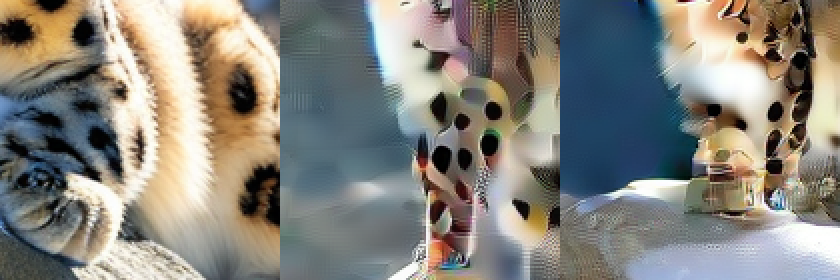
\includegraphics[width=\columnwidth]{figs/qual_crop.png}
\caption{\textbf{Top:} held-out prompts at interval 5. Columns: exact; plain caching;
plain caching $+$ our corrector at the same anchor schedule ($+5.1\%$ FLOPs); and
plain caching at interval 2, which costs $2.1\times$ more FLOPs than either. Per-case
SSIM for these rows goes $0.401\!\to\!0.565$, $0.472\!\to\!0.515$,
$0.428\!\to\!0.482$. Correction restores structure (keyboard, train, animal outline)
but does not approach exact. \textbf{Bottom:} native-resolution crop, $2\times$
nearest-neighbour zoom (exact / plain / corrected). Plain caching imprints a
near-Nyquist cross-hatch over the whole image; the corrector removes most of it and
leaves sparse saturated speckles. This is the comparison that must not be made on
resampled thumbnails: LANCZOS downsampling averages away the grid and preserves the
speckles, reversing the visual impression (Sec.~\ref{sec:artefacts}).}
\label{fig:qual}
\end{figure}

\subsection{An artefact the image metrics do not isolate}
\label{sec:artefacts}

Inspecting outputs at native resolution revealed a failure mode neither SSIM nor LPIPS
separates: plain caching imprints a near-Nyquist cross-hatch over the whole image, at
$8.9\times$ the exact output's energy above $0.8\times$ Nyquist in the LAB lightness
channel, and the corrector halves it to $4.4\times$ while cutting extreme-chroma pixels
from $5.3\%$ to $3.8\%$ (Appendix~\ref{app:artefacts}). We record it because it is a
benefit of correction invisible to the headline metrics, and because it cost us a false
conclusion: viewed in a downsampled contact sheet, LANCZOS resampling averages away the
baseline's near-Nyquist grid while preserving the corrected image's sparse
high-amplitude speckles, exactly reversing the visual impression. Artefact claims in
this setting must be made at native resolution.
